%%%%%%%%%%%%%%%%%%%%%%%%%%%%%%%%%%%%%%%%%%%%%%%%%%%%%%%
%                File: OpEx_temp.tex                  %
%                  Date: Sept. 2, 2009                %
%                                                     %
%           LaTeX template file for use with          %
%           OSA's journal Optics Express              %
%                                                     %
%  send comments to Jennifer Mayfield, jmayfi@osa.org %
%                                                     %
% This file requires style file, opex3.sty, under     %
%              the LaTeX article class                %
%                                                     %
%   \documentclass[10pt,letterpaper]{article}         %
%   \usepackage{opex3}                                %
%                                                     %
% Note that our online submission system does not     %
% currently process PDFLaTeX; if PDFLaTeX must be     %
% used, pls. contact OpEx staff, and we will process  %
% manually                                            %
%                                                     %
%                                                     %
%       (c) 2009 Optical Society of America           %
%%%%%%%%%%%%%%%%%%%%%%%%%%%%%%%%%%%%%%%%%%%%%%%%%%%%%%%

%%%%%%%%%%%%%%%%%%%%%%% preamble %%%%%%%%%%%%%%%%%%%%%%%%%%%
\documentclass[10pt,letterpaper]{article}
\usepackage{opex3}
\graphicspath{{./Pictures/}}
\usepackage{caption}
\usepackage{subcaption}
\usepackage{amsmath} % Required for equation and aligned environments
\usepackage{hyperref}

 %\usepackage{ae} %%for Computer Modern fonts

%%%%%%%%%%%%%%%%%%%%%%% begin %%%%%%%%%%%%%%%%%%%%%%%%%%%%%%
\begin{document}

%%%%%%%%%%%%%%%%%% title page information %%%%%%%%%%%%%%%%%%
\title{Subpixel super resolution algorithm for \textit{PALM microscopy}}

\author{M. Gostiaux Gabriel}

\address{M. Gabriel Gostiaux, Master of Science student, Institute of Optics, \\ Palaiseau, 91 120, France}

\email{gabriel.gostiaux@institutoptique.fr} %% email address is required

\homepage{https://github.com/GabrielGst?tab=repositories} %% author's URL, if desired

%%%%%%%%%%%%%%%%%%% abstract and OCIS codes %%%%%%%%%%%%%%%%
%% [use \begin{abstract*}...\end{abstract*} if exempt from copyright]

\begin{abstract*}
In this study, we introduce a computationally efficient approach for generating super-resolution frames in Photoactivated Localization Microscopy (PALM) by accelerating the processing pipeline. The method is designed to optimize both the localization accuracy and processing speed, making it particularly suitable for medium-large datasets.

\textbf{Keywords:} PALM Microscopy, sub-pixel superresolution, python. 

\end{abstract*}

\ocis{(000.0000) General.} % REPLACE WITH CORRECT OCIS CODES FOR YOUR ARTICLE

%%%%%%%%%%%%%%%%%%%%%%% References %%%%%%%%%%%%%%%%%%%%%%%%%
\begin{thebibliography}{99}

\bibitem{goudail} F. Goudail, ``Fundamental of Estimationa and Detection,'' IOGS {\bf chap. 5,} 59--69 (2023).

\bibitem{labwork} F. Goudail, D. Bloch, O. Leveque, ``FED labworks and projects,'' IOGS {\bf lab 3-4-5,} (2024)

\bibitem{project} T. Molle Heredia, M. Denain, ``Microscopie PALM,'' IOGS {\bf sect. 2.2, 2.3} 4--5, (2023)

\end{thebibliography}

%%%%%%%%%%%%%%%%%%%%%%%%%%  body  %%%%%%%%%%%%%%%%%%%%%%%%%%
\section{Introduction}

PALM (Photoactivated Localization Microscopy) is a high-resolution imaging technique that surpasses the diffraction limit. It relies on the isolation of emitters selectively tagged with a fluorescent molecule, and the fitting of their Point Spread Function (PSF). The fluorescent molecules emit light when stimulated by a laser. This approach enables the precise localization of isolated emitters with an accuracy beyond the Rayleigh criterion, thus providing "super-resolution" down to around 10 nm. This technique, developed by Eric Betzig and his team in 2006, was awarded the Nobel Prize in Chemistry in 2014. It is of great importance due to its ability to enhance the resolution of existing images. Because this method is implemented with noisy frames, one should rely on estimation and detection theory to retrieve the precise coordinates of the emitters.

The workflow begins with a rigorous noise analysis of acquired frames, enabling the subsequent likelyhood computation steps to operate with enhanced precision. Our algorithm leverages a matched filter for likelihood calculation across frames, a critical step in improving computation time.

To accelerate the localization process, we identify initial guesses for molecule positions using a simple peak detection strategy via the numpy.max function. This initial estimation significantly reduces the computational complexity at the cost of sacrificing accuracy. For precise sub-pixel localization, we then employ the Maximum Likelihood Estimator (MLE) method, with optimization executed through the scipy.fmin function. This choice provides a computational efficiency and high-resolution localization, as it can then swiftly converges to optimal coordinates.

\section{Precision analysis}
We have a test image presenting 10 PSF and an array containing the true coordinates of the emitters producing such PSF. In this section we present the analysis of the noise and the influence of the imaging parameters (location of the emitters onto the pixel array and PSF FWHM).

The data used in this study is stored as .mat files which can be loaded in our python environment through the function loadmat of the dependency scipy.io.

\subsection{Noise analysis}

Because the acquired frames are noisy, one should begin by understanding the noise before going forward in the computation of the likelyhood. So, we start by extracting a noisy region of the test image (see Fig. \ref{fig:test}, one could have used a frame from the PALM sequence equivalently), and after flattening the array, we plot it as a 1D signal (see Fig. \ref{fig:noise} and Fig. \ref{fig:noise-1D}).

\begin{figure}[h]
	\centering
	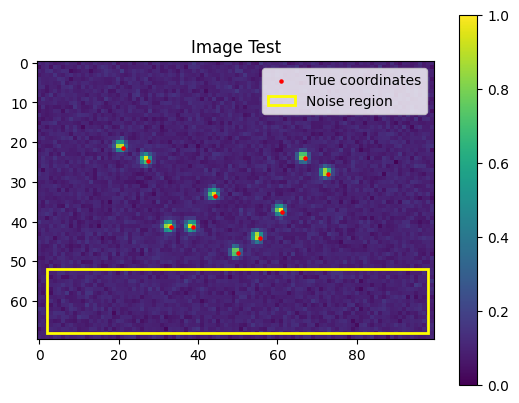
\includegraphics[scale=0.55]{image-test.png}
	\caption{Test Image}
	\label{fig:test}
\end{figure}

This unidimensional signal seems to present a gaussian noise, so we plot a histogram of its values because if we are right, we want to fit a gaussian curve to it to determine its amplitude, mean and standard deviation.

\begin{figure}[h]
     \centering
     \subfloat[Noise]{
         \centering
         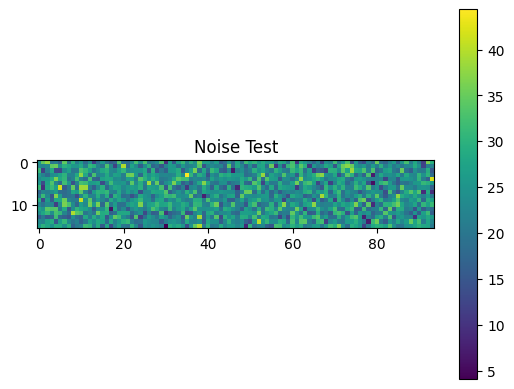
\includegraphics[width=0.45\textwidth]{noise.png}
         \label{fig:noise}
     }
      \subfloat[Noise 1D]{
          \centering
         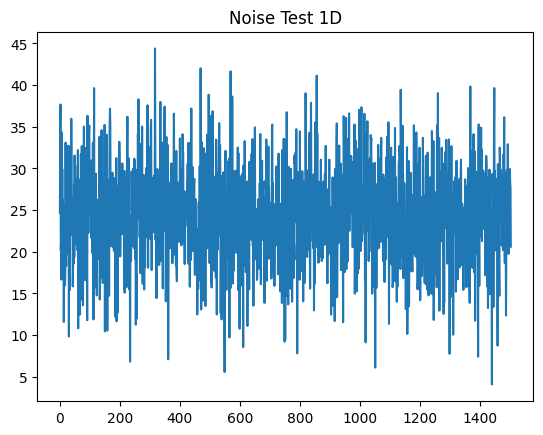
\includegraphics[width=0.45\textwidth]{noise-1D.png}
         \label{fig:noise-1D}
     }
     \caption{Noise}
\end{figure}

The histogram confirms that the noise is gaussian, and we obtain its parameters through the fitted curve: $ [a = 0.06, m = 0.06, \sigma_r = 5.78] $. We then plot the cross correlation of the noise with itself to observe its spatial coherence : since the FWHM length is one (1) pixel, we understand that the noise is white.

\begin{figure}[h]
     \centering
     \subfloat[Noise histogram]{
         \centering
         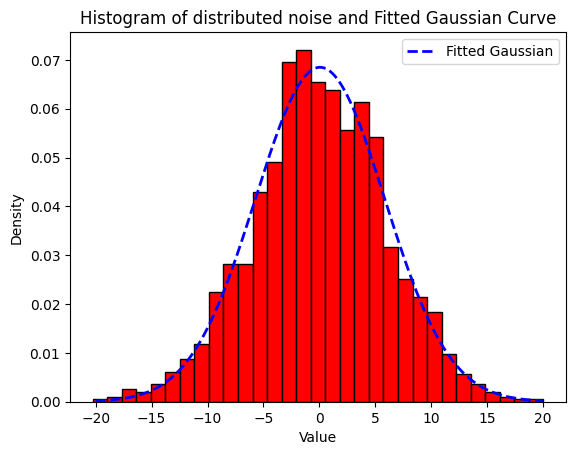
\includegraphics[width=0.45\textwidth]{fitted-gaussian-noise.png}
         \label{fig:fitted}
     }
      \subfloat[Noise correlation]{
          \centering
         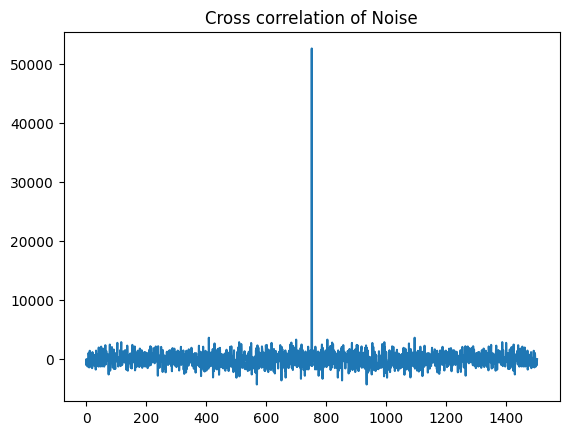
\includegraphics[width=0.45\textwidth]{correlation.png}
         \label{fig:correlation}
     }
     \caption{Noise properties}
\end{figure}

This preliminary analysis concludes that the acquired frames are polluted by a white normal noise of parameters $ [a = 0.06, m = 0.06, \sigma_r = 5.78] $ that will be of use in the computation of likelyhood.

\subsection{Accuracy analysis}\label{accuracy-analysis}

For simplicity reasons and without any loss of generality, we consider the location from a 1D point of view. Let $x$ be the spatial coordinate, $\theta$ the position of an emitter. It is then assumed that the signal given by this single emitter on the image plan can be written as $s(x, \theta)=a r(x, \theta)+b$ where $r$ is a Gaussian function centered on $\theta$ so that

\begin{equation}
     r(x, \theta)=\frac{1}{\sqrt{2 \pi} \sigma_{r}} \exp \left[-\frac{(x-\theta)^{2}}{2 \sigma_{r}^{2}}\right]     
\end{equation}


where $\sigma_{r} = w/(2\sqrt{2ln(2)})$ is expressed as a function of the full width at half maximum (FWHM) $w$ of the signal on the sensor. In this study, $b$ is assumed to be an additive normal white noise of standard deviation $\sigma_{b}$.

We define $r_{i}$ the integration of $r(x, \theta)$ over the pixel $i$ with $i \in[0, N-1]$


\begin{equation}
     r_{i}=\int_{i \Delta x}^{(i+1) \Delta x} r(x, \theta) \mathrm{d} x
\end{equation}


where $\Delta x$ is the discretization step. We can then computes the expression of $r_{i}$ as a function of the parameters $\theta$ and $w$. We remind that


\begin{equation*}
\frac{2}{\sqrt{\pi}} \int_{0}^{z} e^{-u^{2}} \mathrm{~d} u=\operatorname{erf}(z)
\end{equation*}

\pagebreak

Let's compute $r_i$ with a integration by substitution :


\begin{align}
     r_i & =\int_{i \Delta x}^{(i+1) \Delta x} \frac{1}{\sqrt{2 \pi} \sigma_r} \times \exp \left[-\left(\frac{x-\theta}{\sqrt{2} \sigma_r}\right)^2\right] d x \\
     & =\frac{1}{\sqrt{2 \pi} \sigma_r} \times \sqrt{2} \sigma_r \int_{u^{-}}^{u^{+}} e^{-u^2} d u \\
     & =\frac{1}{\sqrt{\pi}}\left[\int_0^{u^{+}} e^{-u^2} d u-\int_0^{u^{-}} e^{-u^2} d u\right]
\end{align}

\begin{align}
r_i= & \frac{1}{2}\left[\operatorname{erf}\left[\frac{(i+1) \Delta x-\theta}{\sqrt{2} \sigma_r}\right]-\operatorname{erf}\left[\frac{i \Delta x-\theta}{\sqrt{2} \sigma_r}\right]\right]
\end{align}

Our goal is to estimate the parameter $\theta_0$ that maximizes the gaussian signal.

\subsection{Position estimation without nuisance parameter: a known}
Here, a is known and equal to 1. The samples are statisticcally independent, they follow a normal probability law described in equation \ref{law} which leads to the expression \ref{log-llh} for the log-likelyhood. We then compute the derivative along $\theta$ to equal expression \ref{MLE} to zero in order to find the estimator of $\theta$, $\hat{\theta}_{ML}$.

\begin{align}
P\left(s_{i}\right) &=\frac{1}{\sqrt{2 \pi} \sigma_b} \exp \left[-\frac{\left(s_i-a r_i\right)^2}{2 \sigma_b^2}\right] \label{law} \\ 
l_\theta &=-N \times ln\left(\sqrt{2 \pi} \sigma_b\right) - \frac{1}{2 \sigma_b^2} \sum_{s_i  \in \Omega} \left(s_i-a r_i\right)^2 \label{log-llh} \\  
\frac{\partial l_\theta}{\partial \theta} &=\frac{1}{\sigma_b^2} \sum_{s_i \in \Omega}\left(s_i-a r_i\right) \times a \times \frac{\partial r_i}{\partial \theta} \label{MLE}
\end{align}

The derivativve let appear the derivative of $r_i$ along $\theta$ which is :

\begin{equation}
     \frac{\partial r_i}{\partial \theta}=-\frac{1}{\sqrt{2 \pi} \sigma_r} \times\left[\exp -\left(\frac{(i+1) \Delta x-\theta}{\sqrt{2} \sigma_r}\right)^2-\exp -\left(\frac{i\Delta x-\theta}{\sqrt{2} \sigma_r}\right)^2\right]
\end{equation}

Because expression \ref{MLE} does not have any analytical solution, we solve it numerically using the fmin function from scipy.optimize dependency. We then choose a parameter $\theta_0 = 41.0050$ to estimate and we evaluate the bias and the variance of its associated estimator $\hat{\theta}_{ML}$ by using a Monte Carlo simulation over 10 000 iterations.

Here we present the results of \cite{project} because ours (produced in lab 3, \cite{labwork}) cannot be computed at the moment of the redaction of this report. The presented bias is $-3.210e-04$ and the presented variance is $2.352e-04$. In regard of the computed bias, we assume the estimator non-biased.

\pagebreak

We then compute the Cramer Rao Lower Bound (CRLB) to see if the variance of the estimator reaches the CRLB. In this case, the estimator $\hat{\theta}_{ML}$ can be defined as efficient. In that purpose, we computes the second derivative of $l_\theta$ along $\theta$ (expression \ref{second-der}) and computes its mean (expressions \ref{CRLB-mean} and \ref{CRLB-mean-2}).

\begin{align}
\frac{\partial^2 l_\theta}{\partial^2 \theta} &=-\frac{1}{\sigma_b^2} \sum_{s_i \in \Omega}\left(-a\left(\frac{\partial c_i}{\partial \theta}\right)^2-\left(s_i-r_i\right) \frac{\partial^2 r_i}{\partial^2 \theta}\right) \label{second-der} \\
\left\langle\frac{\partial^2 l_\theta}{\partial^2 \theta}\right\rangle &=-\frac{1}{\sigma_b^2} \sum_{s_i \in \Omega}\left(-a\left(\frac{\partial r_i}{\partial \theta}\right)^2-\left(\left\langle s_i\right\rangle-\alpha r_i\right) \frac{\partial^2 l_\theta}{\partial^2 \theta}\right) \label{CRLB-mean}\\
\left\langle\frac{\partial^2 l_\theta}{\partial^2 \theta}\right\rangle &=\frac{a}{\sigma_b^2} \sum_{s_i \in \Omega}\left(\frac{\partial r_i}{\partial \theta}\right)^2 \label{CRLB-mean-2}
\end{align}

To obtain the CRLB, we then take the negative inverse of the computed mean to finally get its expression :

\begin{align}
& C R L B=-\frac{\sigma_b^2}{1} \times\left(\sum_{s_i \in \Omega} \left(\frac{\partial r_i}{\partial \theta}\right)^2\right)^{-1} \\
& C R L B=2\pi\sigma_b^2\sigma_r^2 \times\left(\sum_{s_i \in \Omega}\left(e^{-u_+^2}-e^{-u_{-}^2}\right)^2\right)^{-1}
\end{align}

\begin{figure}[h]
	\centering
	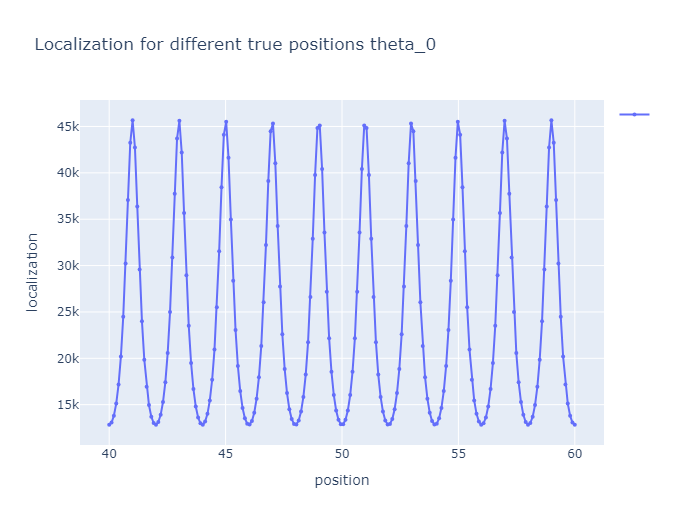
\includegraphics[scale=0.45]{CRLB_evol.png}
	\caption{CRLB as a function of $\theta$}
	\label{fig:CRLB-evol}
\end{figure}

The result presented in the study is $2.568e-04$ so that we conclude the estimator is efficient \cite{project}. Because the estimator is non-biased and because it belongs to the exponential family, one could have predicted thoses results \cite{goudail}.

\subsection{Position estimation with nuisance parameter: a unknown}
In the case where a is unknown, one should first estimate its value in order to estimate the location ($\theta$). We set $a$ as a parameter in the expression of the log-likelyhood.
\begin{equation}
l(a, \theta)=-N \ln \left(\sqrt{2 \pi} \sigma_b\right)-\frac{1}{2 \sigma_b^2} \sum_{i=0}^{N-1}\left(s_i-a r_i\right)^2
\end{equation}

We then computes the derivative along $a$ to find the MLE $\hat{a}_{ML}$ :
\begin{equation}
     \left.\frac{\partial l}{\partial a}\right|_{a-\hat{a}_{M L}}=\frac{1}{\sigma_b^2} \sum_{i=0}^{N-1} r_i(\theta)\left(s_i-\hat{a}_{M L} r_i(\theta)\right)=0
\end{equation}

We get :
\begin{equation}
     \hat{a}_{M L}=\frac{\sum_{i=0}^{N-1} s_i r_i(\theta)}{\sum_{i=0}^{N-1} r_i(\theta)^2}
\end{equation}

Now, we inject this expression in equation \ref{log-llh}. As before, we solve it numerically. We then choose a parameter to estimate and we evaluate the bias and the variance of its associated estimator $\hat{\theta}_{ML}$ by using a Monte Carlo simulation over 10 000 iterations.
Again (and for the same reasons as mentioned above), we present here the results of \cite{project}. The measured bias $6.998e-05$ is and the measured variance is $2.424e-04$. Again, the estimator is non biased, and because it belongs to the exponential family, we expect it to reach the CRLB.

In this mean, we start by computing the Fisher Information matrix :

\begin{equation}
     I(a, \theta)=\left[\begin{array}{ll}
          A & B \\
          C & D
          \end{array}\right]
\end{equation}

With the following coefficients :

\begin{align}
     & A=\frac{1}{\sigma_b^2} \sum_{i=0}^{N-1} r_i(\theta)^2 \\
     & B=\frac{1}{\sigma_b^2} \sum_{i=0}^{N-1} \hat{a}_{M L} r_i(\theta) \frac{d r_i}{d \theta} \\
     & C=B \\
     & D=\frac{1}{\sigma_b^2} \sum_{i=0}^{N-1} \hat{a}_{M L}^2\left[\frac{d r_i}{d \theta}\right]^2
\end{align}

Because $I(a, \theta)$ is invertible \cite{goudail}, we compute $J(a, \theta) = I(a,\theta)^{-1}$. The CRLB is given by the coefficient (2,2) of matrix $J$, so that :

\begin{equation}
     CRLB(\theta) = \frac{A}{AD-BC}
\end{equation}

The results presented in \cite{project} suggest that no matter the knownledge of a, the estimator $\hat{\theta}_{ML}$ is efficient.

\pagebreak

\section{Implementation of the algorithm}

We have a sequence of 999 frames each containing 10 PSF spreaded over the frame. We are presented with the 999 frames overlayed so that it produces a blurred image (see Fig. \ref{fig:floue}) which seems to be a text. Our goal is to extract precisely the locations of the emitters producing the PSF and to arrange them into a super-resoluted grid (say 10 times wider).

\begin{figure}[h]
	\centering
	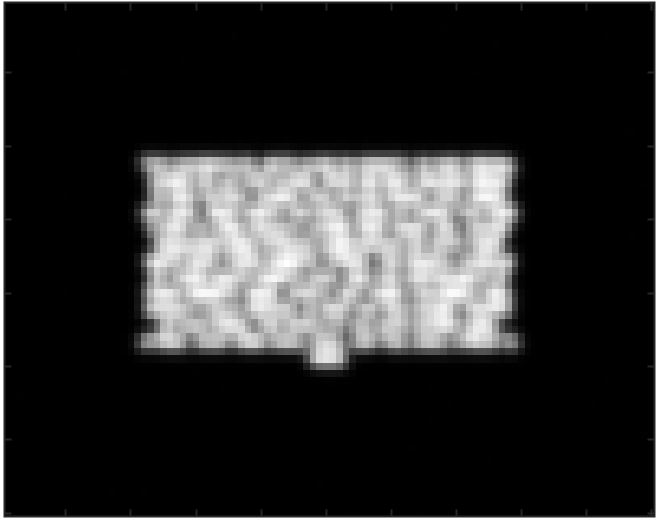
\includegraphics[scale=0.65]{ImageFloue.JPG}
	\caption{Image floue}
	\label{fig:floue}
\end{figure}

To compute the Maximum Likelyhood Estimator (MLE), one should first define the model function. Here, it will be a two-dimensional gaussian function as defined in 1D in subsection \ref{accuracy-analysis}. Thus, we have the following model function, after pixel-wide integration :

\begin{equation}
\begin{aligned}
r_{i j}\left(\theta_x, \theta_y\right)=\frac{1}{4}&\left[\operatorname{erf}\left(\frac{(i+1)-\theta_x}{\sqrt{2} \cdot \sigma_r}\right)-\operatorname{erf}\left(\frac{i-\theta_x}{\sqrt{2} \cdot \sigma_r}\right)\right] \\
& \times\left[\operatorname{erf}\left(\frac{(j+1)-\theta_y}{\sqrt{2} \cdot \sigma_r}\right)-\operatorname{erf}\left(\frac{j-\theta_y}{\sqrt{2} \cdot \sigma_r}\right)\right]
\end{aligned}
\end{equation}

With that in mind, we can proceed to compute the log-likelyhood :

\begin{equation} \label{log-likelyhood}
     l\left(\theta_x, \theta_y\right)=-I \cdot J \cdot \ln \left(\sqrt{2 \pi} \sigma_b\right)-\frac{1}{2 \sigma_b^2} \sum_{i=0}^{I-1} \sum_{j=0}^{J-1}\left(s_{i j}-a r_{i j}\right)^2
\end{equation}

This function will unravel its full capacity when adressing the optimization step. However, in regard to the computation time improvement, we will proceed in computing the log-likelyhood through the ambiguity function using the matched filter. The matched filter, computed as a correlation in Fourier's domain between a model function centered in its frame and the 999 acquired images, is 10 times faster than the numerical computation with the analog expression of equation \ref{log-likelyhood}.

We can then export the 999 log-likelyhood arrays to import them later. They will be refered to as frames from now on.

On each frame, we first locate the 10 pixel-scale global maxima and store them in a list as initial guesses for the solving function. Then, we use the fmin solving function from scipy.optimize module to locate the local maxima in a sub-pixel scale. This workflow allows to compute the log-likelyhood function according to its analog expression only in a neighbourhood of the global maxima, which significantly reduces the computation time. We plot the initial guesses and the super-resoluted emitters coordinates on Fig. \ref{fig:eval}.


\begin{figure}[h]
	\centering
	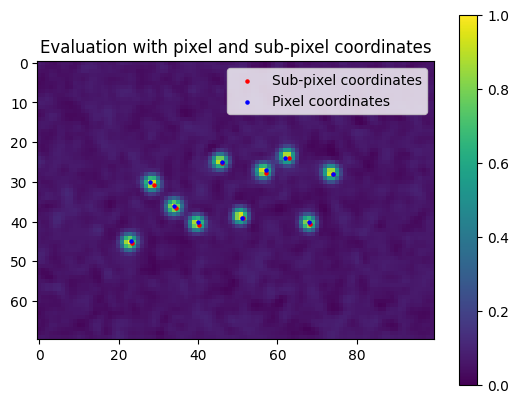
\includegraphics[scale=0.65]{evaluation of algo.png}
	\caption{Evaluation of algorithm acccuracy}
	\label{fig:eval}
\end{figure}

The coordinates seems relevant in a significant subset of the acquire image, therefore we decide now to proceed to the analysis of the 999 acquired images. On Fig. \ref{fig:pix}, one could recognize the shape of the blurred image, suggesting that the maxima should be well computed (at pixel scale and therefore at sub-pixel scale too). Fig. \ref{fig:subpix} shows reconstruction on its way\dots

\begin{figure}[h]
     \centering
     \subfloat[Initial guesses]{
         \centering
         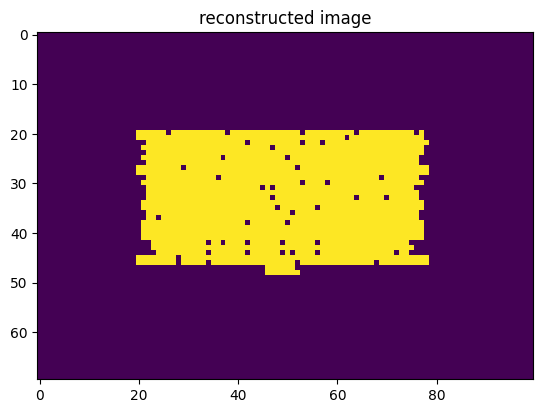
\includegraphics[width=0.45\textwidth]{pix-sum.png}
         \label{fig:pix}
     }
      \subfloat[Solving...]{
          \centering
         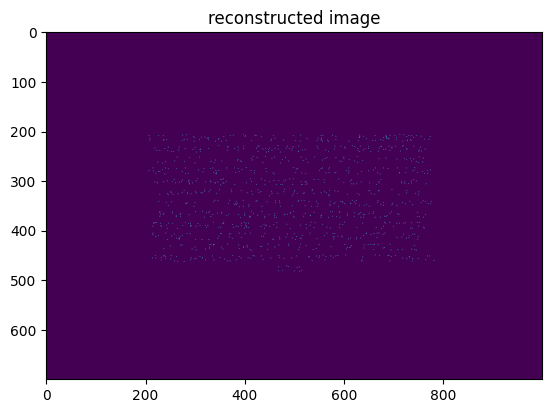
\includegraphics[width=0.45\textwidth]{solving-1.png}
         \label{fig:subpix}
     }
     \caption{Computing pix and subpix coordinates}
\end{figure}

The algorithm finally produces Fig. \ref{fig:super} on which one could read a passage of the famous "Romeo and Juliette" piece written by M. William Shakespeare. This proves the described fast-algorithm still produces super-resoluted frames without significant loss in accuracy compared to the basic ones. The figure was produced in fifteen (15) minutes total, including five (5) minutes of log-likelyhood computation and export, and ten (10) minutes of super-resolution estimation, on custom desktop hardware including intel core i7 14700KF processor and NVIDIA RTX 4060 Ti 8Gb graphic card (which was not used for computation).

\begin{figure}[h]
	\centering
	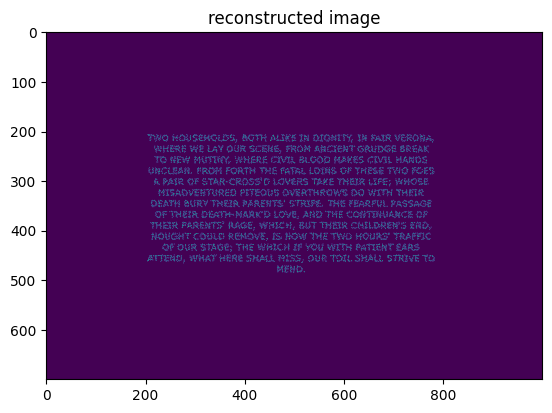
\includegraphics[scale=0.65]{solved text.png}
	\caption{Super resolution image}
	\label{fig:super}
\end{figure}

\section{Conclusion}
This study presented a specific workflow to optimize computation time for PALM microscopy. The proposed method consist in using a matched filter to compute and save the log-likelyhood arrays from the acquired frames, then use the numpy max function on those to find pixel-wide initial guesses for the scipy fmin optimization function. The time efficiency is then improved by a factor of 10, leading to compute the super-resoluted image presented at the end of section 2 in 10 minutes, while it was expected to be computed in 100 minutes with the basic fmin MLE optimization method.

The workflow produces a super-resoluted image on which one could read a passage of the famous "Romeo and Juliette" piece written by M. William Shakespeare, proving the accuracy of the method.

\listoffigures

\end{document} 
